\documentclass[a4paper,oneside,11pt]{scrreprt}
\usepackage{scrhack} % to suppress warning

% include style from other file
\usepackage{style}

\begin{document}

\pagenumbering{gobble}

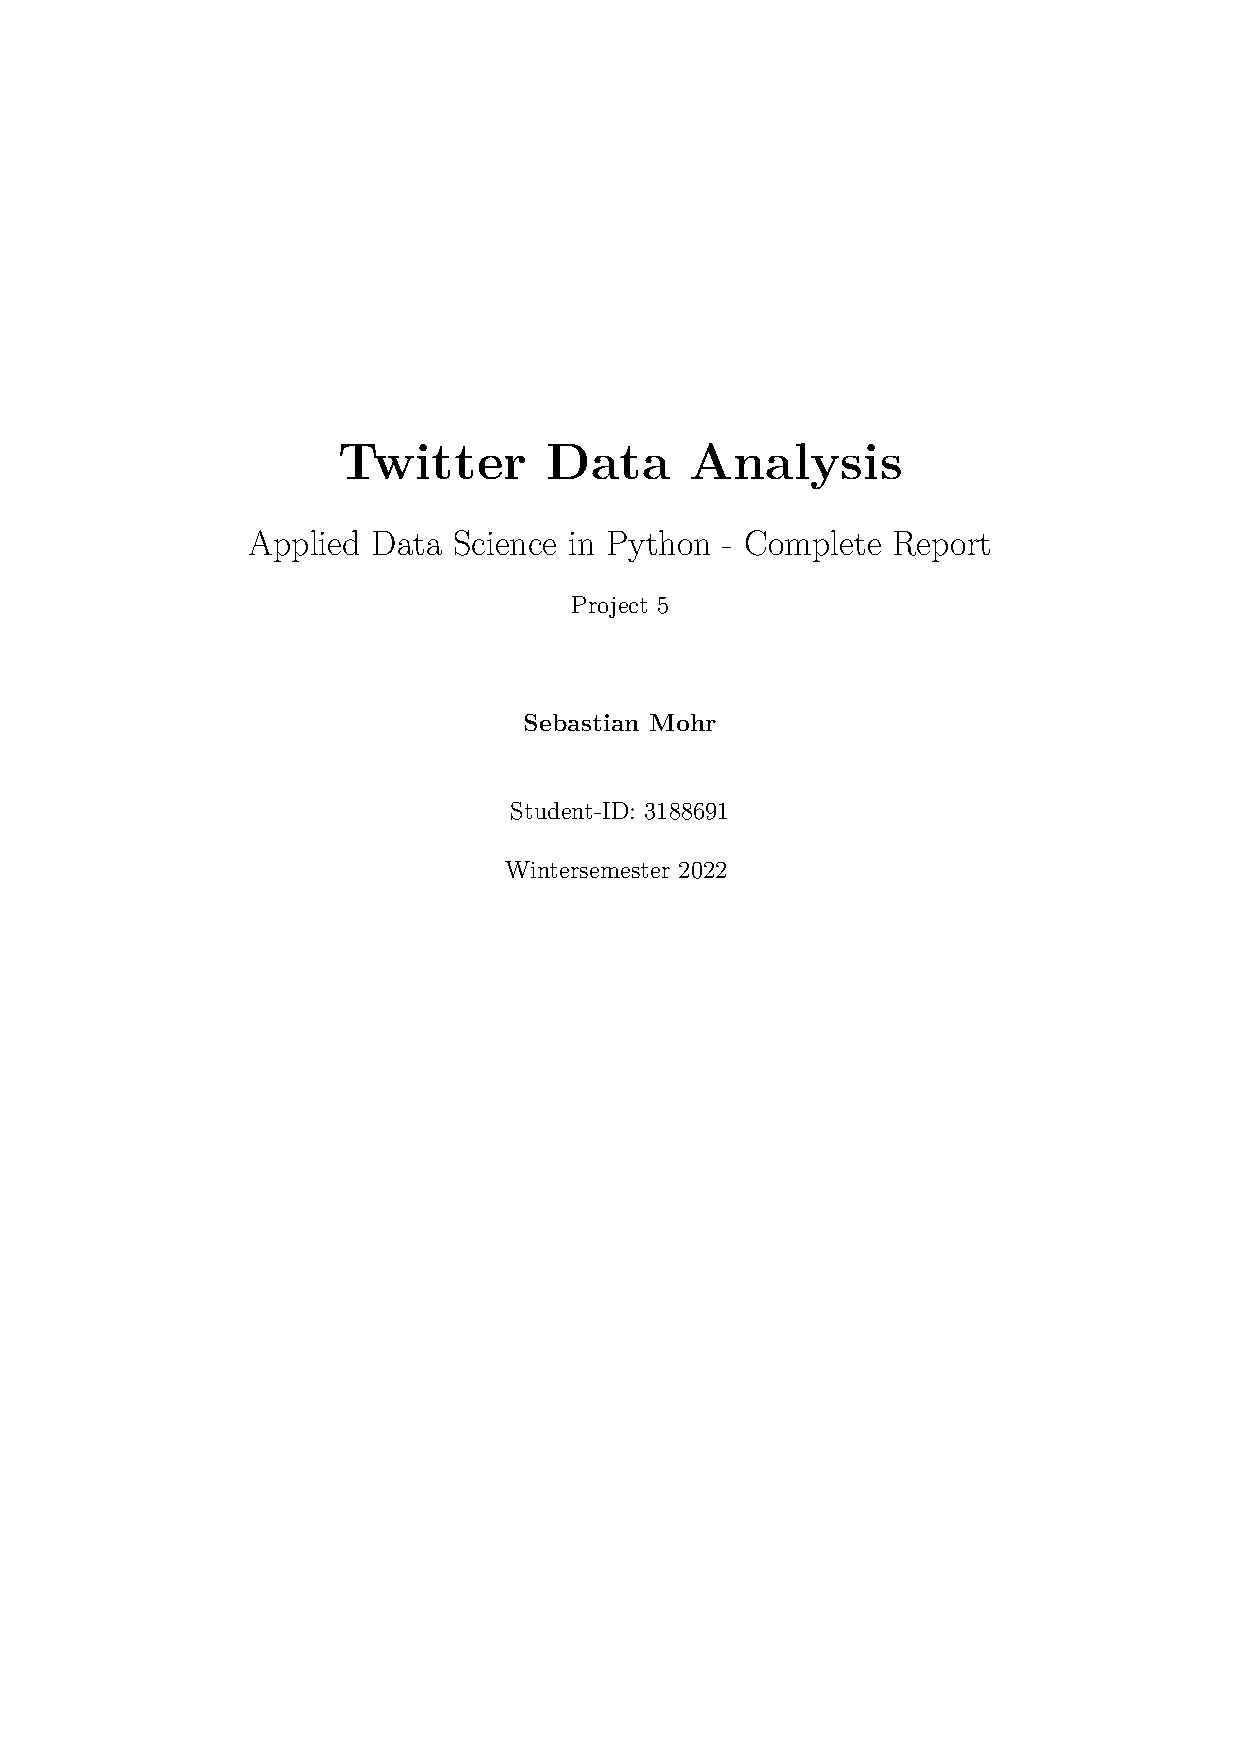
\includepdf{cover.pdf}

\newpage

\pagenumbering{arabic}

\chapter{Project Description}
The goal of this project is to give users the ability to get information about a specific events hashtag and its top conversations on \requirement{Twitter}. The tweets for an event should be analyzed and the sentiment displayed for the user of the application. Additionaly the application shows the Top 10 hashtags and users associated with the chosen event. The user can further investigate the displayed data and look at the users, as well as their followers and the tweets.

\section{Modules, data structure, tools}

In this section I will explain how I accessed the data I needed for my application and how I structured the data. Also I will define which Tools, Application, Modules and IDE I used in the course of this project.

\subsection{Getting the data}

The data that will be shown in the application will be gathered through the Twitter developer API. To achive this I signed up to Twitter with a new account that registered for the developer tools. Twitter already provides libraries for Python to easiely access its API.\\

First the app has to authenticate itself, to make sure that it is connected to the already created Twitter account. After the authentication the data can be gathered through a search url, that contains all the query parameters. Here the search url tells the API which data the application wants to get. The query parameters specify different metrics for the tweets, like the tweet author, date and time of its creation or used hashtags.\\

For this problem the API call will first retrieve all tweets that contain the hashtag of the searched for event. After analyzing the tweets, the the Top 10 contributors account data will also be retrieved from the API.

\subsection{Data structuring}

The data provided by the Twitter API has to be processed somewhere in memory. To achive this goal, the data will be saved into objects of the \requirement{pandas} type \code{DataFrame}. \code{DataFrame}s have the advante of being able to store and filter large amounts of data in memory. Additionaly it can be easily exported to CSV. When saving the data on the hard drive it can be accessed every time when opening the application and only be updated when it is requested. This will boost the performance of the application, as it's not dependent on an internet connection for basic features and doesn't have to gather new data on every startup. The data can then still be updated in the background when clicking an update button for example. The application handles tweets and users, which will be saved in seperate \code{DataFrame}s.

\subsection{Tools and Application}

The backend of the application will be written in \code{Python}, as it provides good data analysing tools for the different problems of this project. To access the Twitter API I will use the \code{Tweepy} library. \code{Tweepy} provides several features to use all of the methods the Twitter API offers. For the \requirement{sentiment analysis} I will use the python library \code{TextBlob}. It's a text processing library which helps to analyze written text, which is perfect for analyzing many written tweets about a specific topic like a big event.\\

For the frontend I will use a web application, which will use several different \code{TypeScript} files. In these files I will build a User Interface with the library \code{React}. With \code{React} interactive web pages can be build that behave like a native running program would. To power \code{React} I will use \code{MUI} as the component library.

\subsection{Modules and Algorithm}

The application will be split between front- and backend. In the frontend, only the user interface and basic computation, while the backend will handle all the Twitter API calls, as well as the data processing and persistence. \\

The application will first gather a specific number of tweets for the event from the Twitter API. After saving and analyzing the data, the Top 10 users by interactions will be figured out. Their info will also be retrieved from the Twitter API. After one of the Twitter users is clicked, its profile will be retrieved from Twitter and its followers and information will be displayed. The followers als can be viewed and their tweets will also be retrieved from the Twitter API.

\subsection{IDE}

To develop the application I used two IDEs from JetBrains. For the Python backend I used the PyCharm IDE, as it provides good features like automatic imports and code completion. The same can be said for WebStorm, which I used to develop the frontend. Both of the IDEs have the same keybindings and plugins, which makes it very easy to work with both of them at the same time.


\chapter{High Level Design}
The application is split between front- and backend. The backend handles most of the data loading, transformation and persistence. To get the data from the backend, it runs on a simple Web-Api, that provides a few endpoints where data can be accessed. The frontend then calls these endpoints and retrieves the data through JSON objects, which can be easily deserialized in the frontend application and then displayed to the user.

The backend provides 6 different endpoints:

\begin{itemize}
    \item \requirement{/api/sentiment}: The most important endpoints. When this endpoint is called, the backend retrieves tweets for a specific hashtag (given as query parameter), then analyzes them and sends them back to the frontend.
    \item \requirement{/api/top}: This frontend automatically gets called after the sentiment analysis has been retrieved. The backend analyzes the recently retrieved tweet-list and searches for the most used hashtags and the users with the most tweets in the data set.
    \item \requirement{/api/user}: This endpoint is used to get information about one user. The backend receives information of the user with the given user-id from the twitter API. Metrics like follower-count, following-count and so on are contained in the retrieved data set.
    \item \requirement{/api/user/followers}: This endpoint returns a list of up to 100 followers of the given user.
    \item \requirement{/api/user/tweets}: This endpoint returns a list of the most recent tweets of the given user.
    \item \requirement{/api/hashtag}: With this endpoint, all the tweets that contain both the main-hashtag and one of the top hashtag can be retrieved from the backend.
\end{itemize}

\begin{figure}[H]
    \centering
    \caption{Flowchart of the application design}
    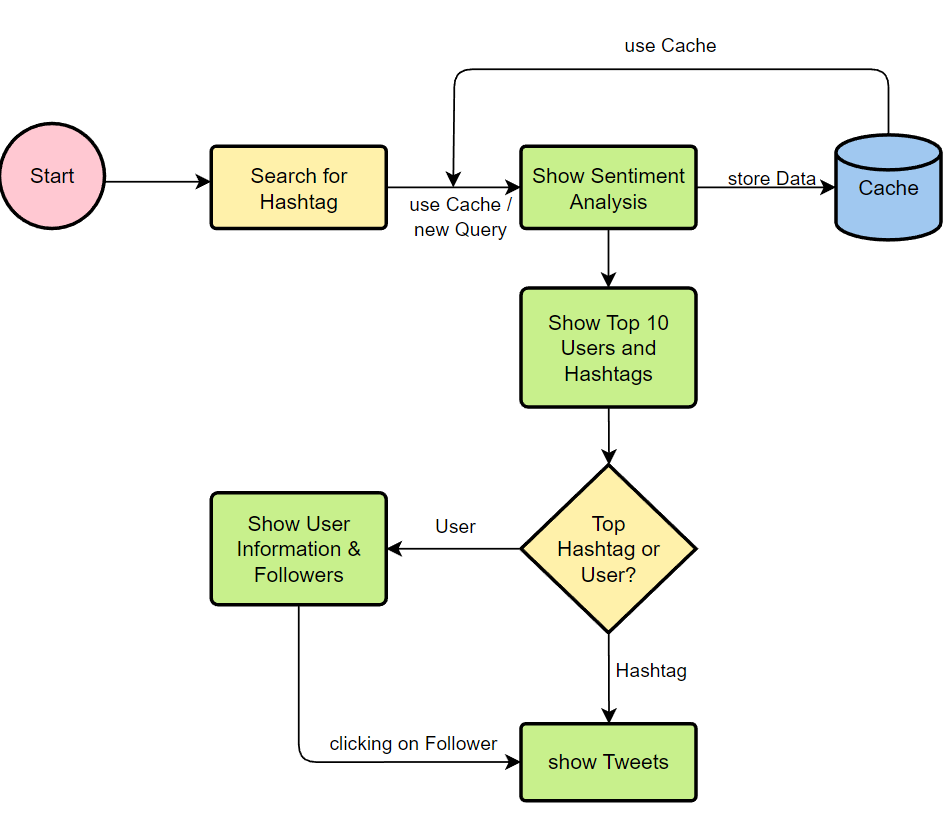
\includegraphics[width=\textwidth]{media/2_Design.png}
\end{figure}

\section{Necessary Functions}

The application has some necessary functions for each problem.

\begin{itemize}
    \item \requirement{TweepyClient}: I created a class named \code{TweepyClient} to have all the necessary functions used for communicating with the Twitter API in one class. Here you can find the functions \code{GetTweetsByHashtag(hashtag, max\_results)}, \code{GetFollowers\-ByUserId(user\_id)}, \code{GetUserMetricsByUserId(user\_id)} and \code{GetTweetsFromUser\-Id(user\_id)} that include the basic Twitter API requests for each endpoint.
    \item \requirement{AnalyseSentimentOfTweetList()}: This function is part of the \code{SentimentAnalyzer} class, that includes a tweet-list as parameter. The analysis method takes this list and analyzes every tweet in the list with the help of the \code{TextBlob}-library. Then the Tweet-objects get assigned their sentiment. The tweet-list afterwards get returned to the caller.
    \item \requirement{AnalyzeTweetList()}: This method is part of the \code{TopHashtagsAndUsersAnalyzer} class, which includes a tweet-list and the main hashtag as attributes. The function is used to find the most used hashtags and the users with the most tweets in the analyzed data set. It returns a tuple of two lists, one containing the top hashtags and the other containing the top users.
    \item \requirement{StringValidator}: This class is used to validate the strings before making any data transformations. As the API can possibly also be accessed from outside of the frontend, there could be malicious requests, which can be prevented when validating query parameters before accessing data.
    \item \requirement{CsvHelper} and \requirement{TweetDataframeHelper}: These two classes were used to unify and ease the work with DataFrames and cached CSV-Data. Whenever the cache has to be accessed, the CsvHelper class was used, so that there is only one place where data is written and read in the application. The TweetDataframeHelper was used to write the Tweet-list into a dataframe or read it frome a given Dataframe and return it to the caller as list.
\end{itemize}

\chapter{User Interface}
The user interface was programmed in React and thus is a single page application. The necessary fragments of the application always get shown/hidden when needed.

\begin{figure}[H]
    \centering
    \caption{Starting Screen with parameter selection}
    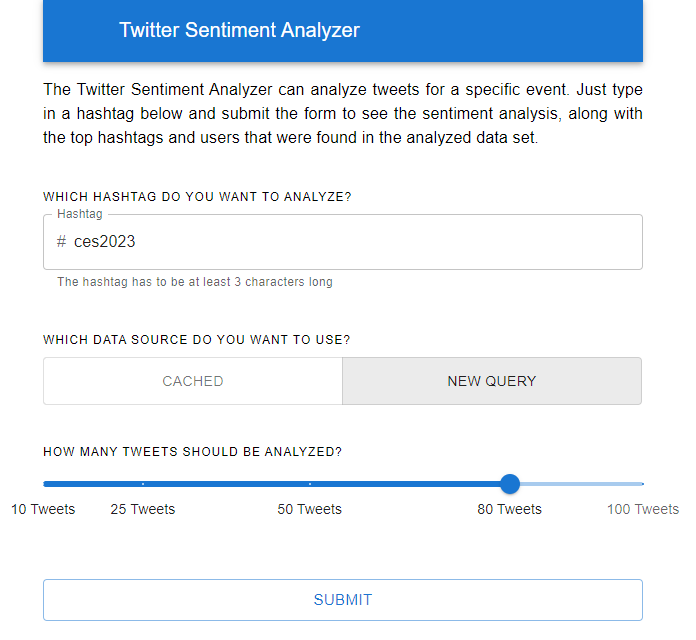
\includegraphics[width=\textwidth]{media/3_StartScreen.png}
\end{figure}

\begin{figure}[H]
    \centering
    \caption{Sentiment Screen with sentiment analysis and Top Hashtags / Users}
    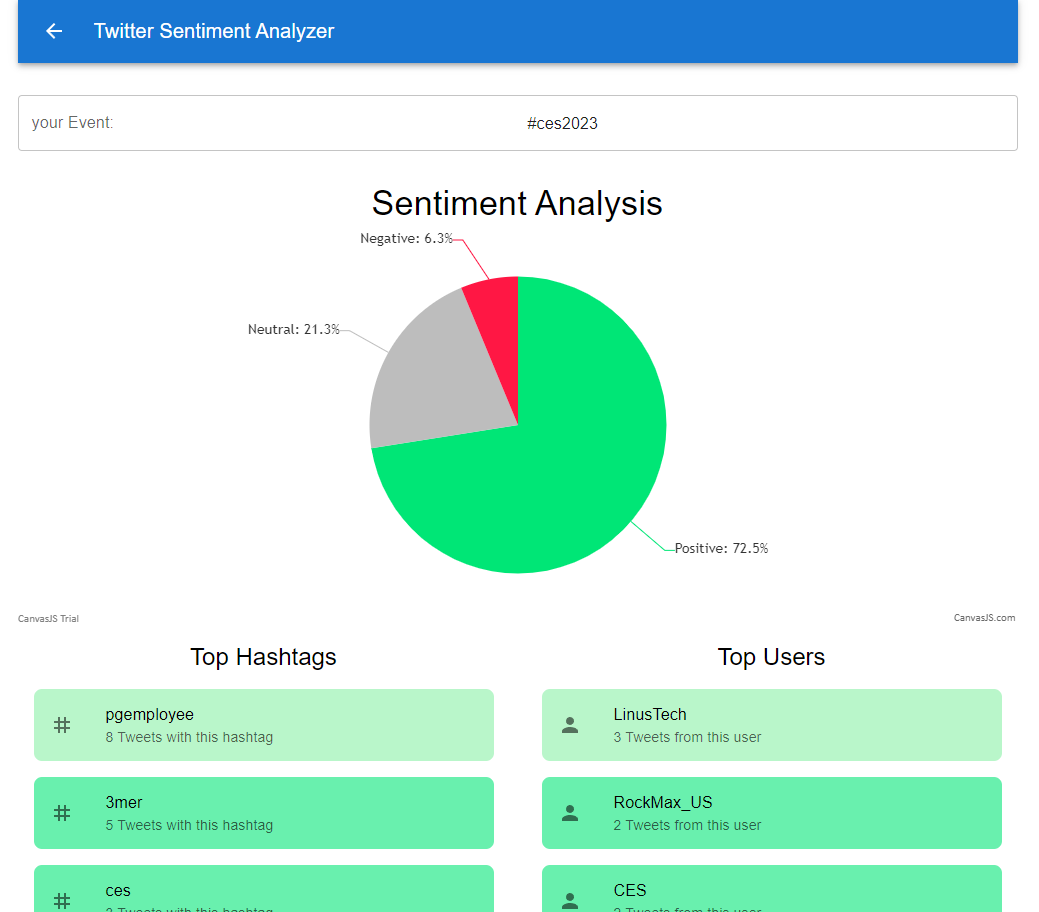
\includegraphics[width=\textwidth]{media/3_SentimentScreen.png}
\end{figure}

\begin{figure}[H]
    \centering
    \caption{User Dialog with basic information}
    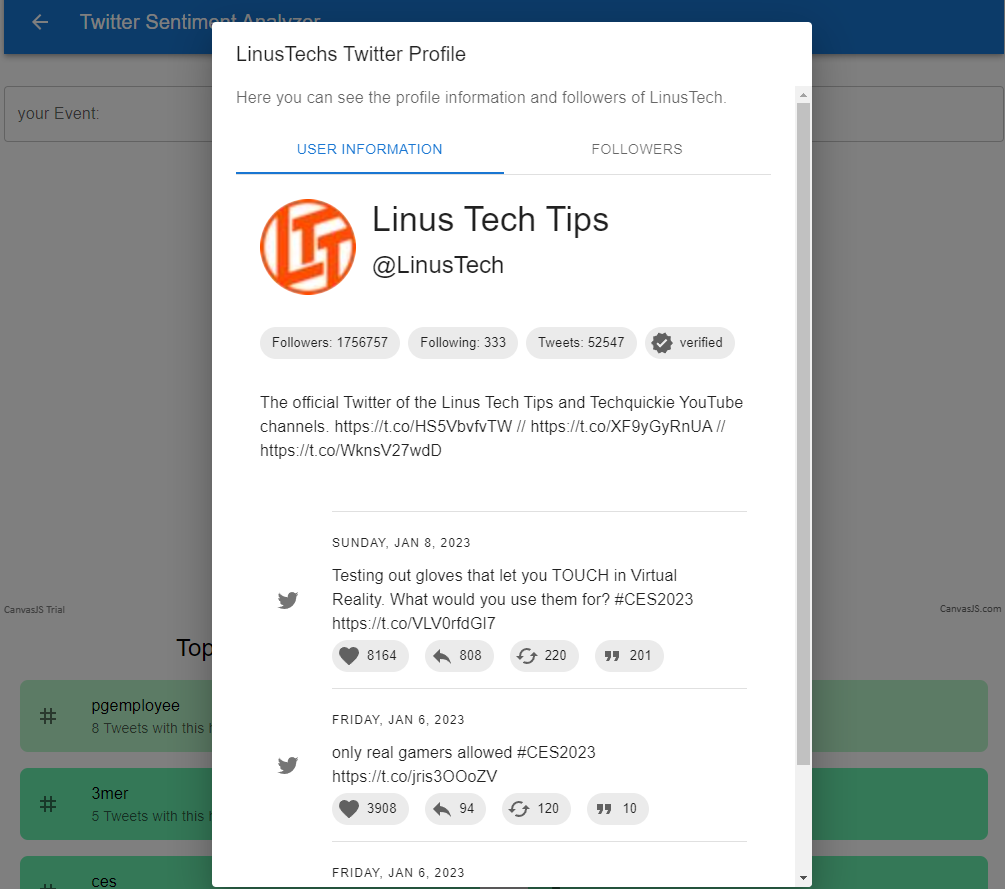
\includegraphics[width=0.75\textwidth]{media/3_UserScreen.png}
\end{figure}

\begin{figure}[H]
    \centering
    \caption{User Dialog with followers}
    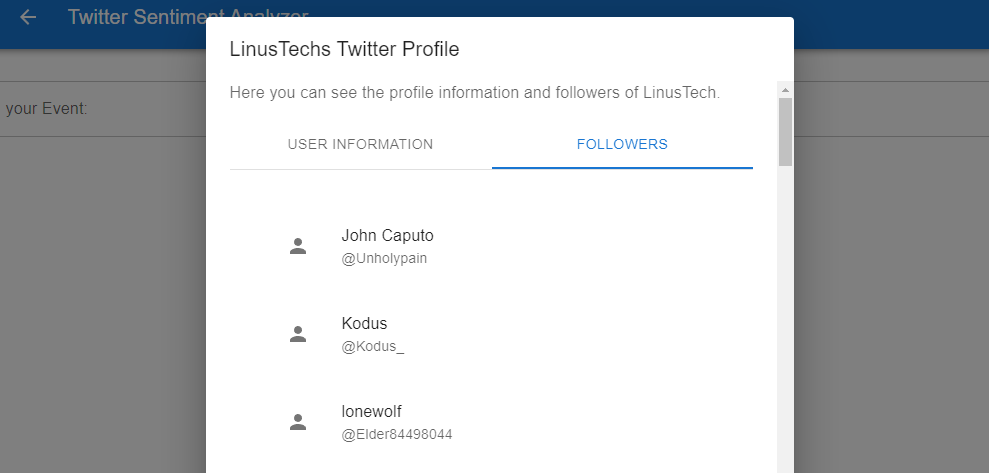
\includegraphics[width=0.75\textwidth]{media/3_FollowersScreen.png}
\end{figure}

\begin{figure}[H]
    \centering
    \caption{Tweet Dialog of followers tweets}
    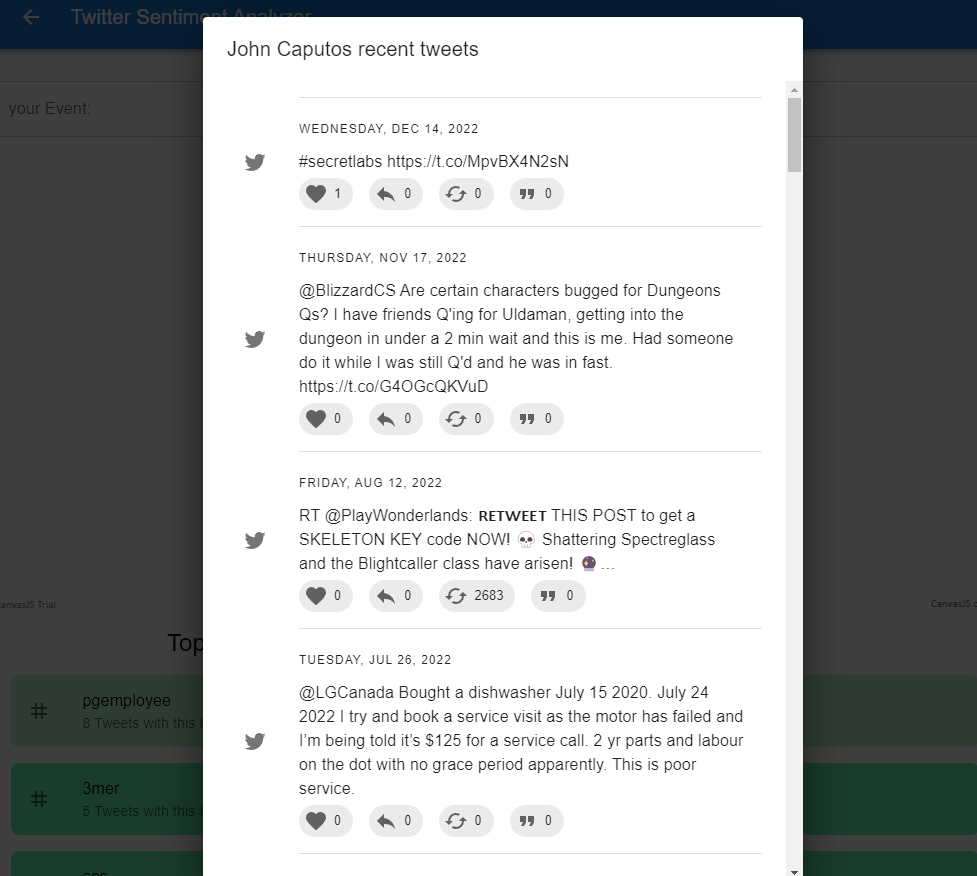
\includegraphics[width=0.75\textwidth]{media/3_FollowersTweetsScreen.png}
\end{figure}

\begin{figure}[H]
    \centering
    \caption{Tweet Dialog of tweets that include the selected hashtag}
    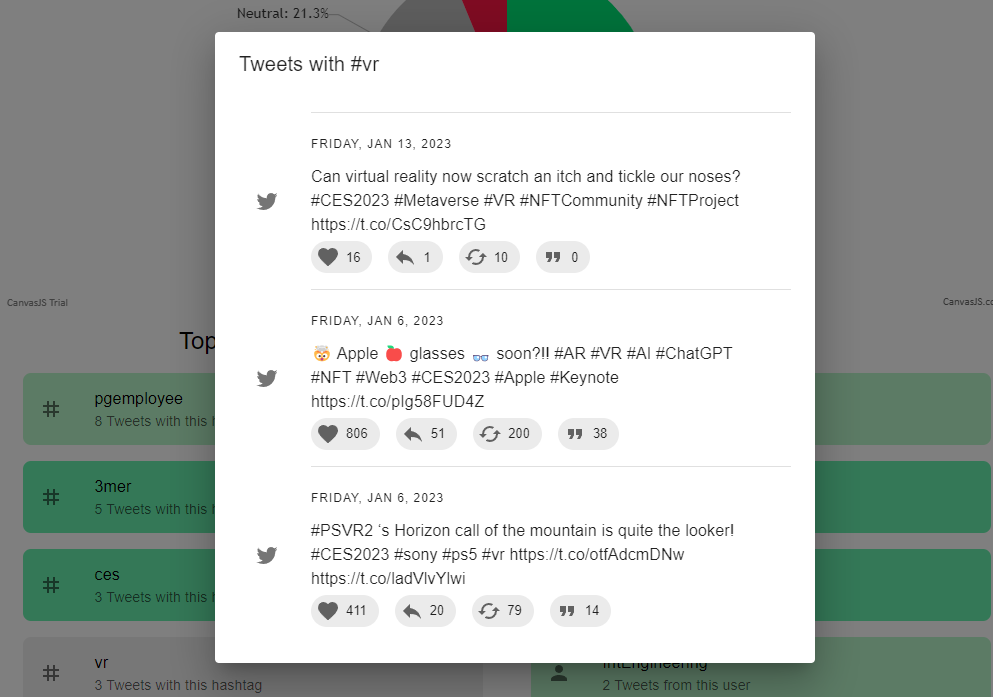
\includegraphics[width=0.75\textwidth]{media/3_HashtagTweetsScreen.png}
\end{figure}

The cached data was saved in a CSV-file, which includes all the analyzed Tweets Data, but no data from the users except the author\_id:

\begin{figure}[H]
    \centering
    \caption{Example data for \#CES2023}
    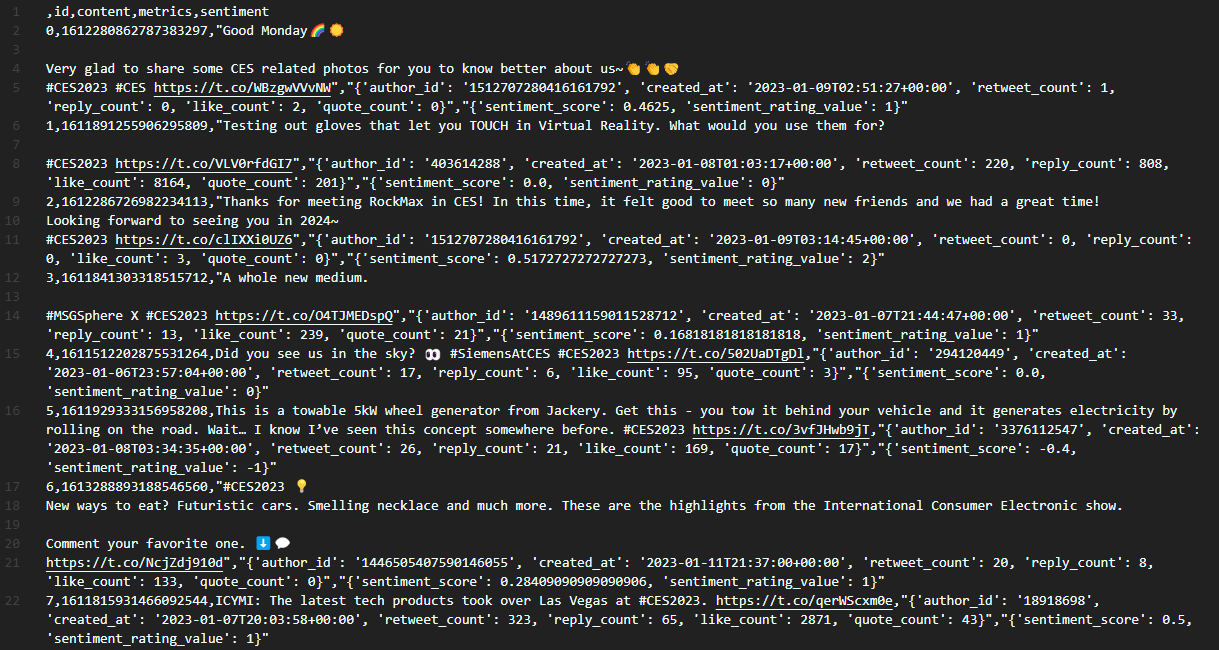
\includegraphics[width=\textwidth]{media/3_CSV.png}
\end{figure}


\chapter{Conclusion}

After working on this project for the past couple weeks, I can say that data science is not as easy as I have thought. Often the data doesn't behave like I would like it to. I often ran into problems where my backend provided the data not like my frontend requested it and so there where a few exceptions that I had to overcome. All in all I'm proud of the application I developed and it was fun working on my own project. I learned a few things about Python, Pandas, API-requests and Frontend development. Sadly I wasn't able to use machine learning in this project, but its a topic I want to work on in the future and am in anticipation of learning.

\end{document}